\begin{minipage}{0.75\linewidth}
\begin{figure}[h]
    \centering
    \begin{adjustbox}{max width=1.0\linewidth, keepaspectratio}
        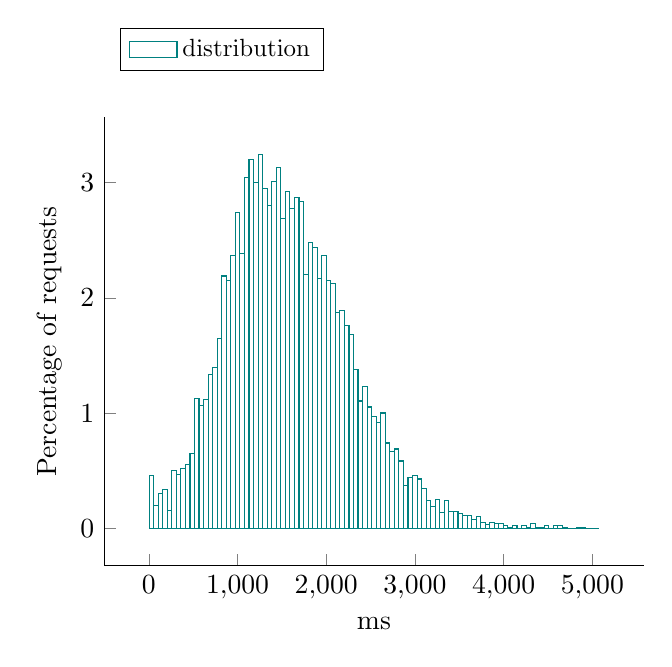
\begin{tikzpicture}
            \begin{axis}[ylabel = Percentage of requests, 
xlabel = ms, 
legend style = {nodes={scale=0.9, transform shape}, at={(0.03,1.2)}, anchor=north west, draw=black, fill=white, align=left, legend columns=3},
area style, mark size = 0pt,
 cycle list name = exotic,
  axis lines* = left]
		\addplot +[ybar interval] coordinates {
			 (3, 0.458811)
			 (54.21, 0.198123)
			 (105.42, 0.302398)
			 (156.63, 0.333681)
			 (207.84, 0.156413)
			 (259.05, 0.500521)
			 (310.26, 0.469239)
			 (361.47, 0.521376)
			 (412.68, 0.552659)
			 (463.89, 0.646507)
			 (515.1, 1.12617)
			 (566.31, 1.06361)
			 (617.52, 1.11575)
			 (668.73, 1.33472)
			 (719.94, 1.39729)
			 (771.15, 1.64755)
			 (822.36, 2.18978)
			 (873.57, 2.14807)
			 (924.78, 2.36705)
			 (975.99, 2.74244)
			 (1027.2, 2.3879)
			 (1078.41, 3.04484)
			 (1129.62, 3.20125)
			 (1180.83, 3.00313)
			 (1232.04, 3.24296)
			 (1283.25, 2.95099)
			 (1334.46, 2.80501)
			 (1385.67, 3.01356)
			 (1436.88, 3.12826)
			 (1488.09, 2.6903)
			 (1539.3, 2.91971)
			 (1590.51, 2.77372)
			 (1641.72, 2.86757)
			 (1692.93, 2.83629)
			 (1744.14, 2.20021)
			 (1795.35, 2.48175)
			 (1846.56, 2.44004)
			 (1897.77, 2.16893)
			 (1948.98, 2.36705)
			 (2000.19, 2.14807)
			 (2051.4, 2.12722)
			 (2102.61, 1.87696)
			 (2153.82, 1.88738)
			 (2205.03, 1.76225)
			 (2256.24, 1.67883)
			 (2307.45, 1.37643)
			 (2358.66, 1.10532)
			 (2409.87, 1.23045)
			 (2461.08, 1.05318)
			 (2512.29, 0.96976)
			 (2563.5, 0.917623)
			 (2614.71, 1.00104)
			 (2665.92, 0.740355)
			 (2717.13, 0.667362)
			 (2768.34, 0.688217)
			 (2819.55, 0.583942)
			 (2870.76, 0.375391)
			 (2921.97, 0.437956)
			 (2973.18, 0.458811)
			 (3024.39, 0.427529)
			 (3075.6, 0.344108)
			 (3126.81, 0.239833)
			 (3178.02, 0.187696)
			 (3229.23, 0.250261)
			 (3280.44, 0.135558)
			 (3331.65, 0.239833)
			 (3382.86, 0.145985)
			 (3434.07, 0.145985)
			 (3485.28, 0.12513)
			 (3536.49, 0.114703)
			 (3587.7, 0.114703)
			 (3638.91, 0.0729927)
			 (3690.12, 0.104275)
			 (3741.33, 0.0521376)
			 (3792.54, 0.0312826)
			 (3843.75, 0.0521376)
			 (3894.96, 0.0417101)
			 (3946.17, 0.0417101)
			 (3997.38, 0.0208551)
			 (4048.59, 0.0104275)
			 (4099.8, 0.0208551)
			 (4151.01, 0)
			 (4202.22, 0.0208551)
			 (4253.43, 0.0104275)
			 (4304.64, 0.0417101)
			 (4355.85, 0.0104275)
			 (4407.06, 0.0104275)
			 (4458.27, 0.0208551)
			 (4509.48, 0)
			 (4560.69, 0.0208551)
			 (4611.9, 0.0208551)
			 (4663.11, 0.0104275)
			 (4714.32, 0)
			 (4765.53, 0)
			 (4816.74, 0.0104275)
			 (4867.95, 0.0104275)
			 (4919.16, 0)
			 (4970.37, 0)
			 (5021.58, 0)
			 (5072.79, 0)
		};
\addlegendentry{distribution};
           \end{axis}
      \end{tikzpicture}
  \end{adjustbox}
  \caption{Response time distribution - req = ReadUser-3}
\end{figure}
\end{minipage}\hfill\begin{minipage}{0.18\linewidth}
\begin{table}[h]
\begin{tabular}{|cc|}
\hline
\textbf{} & \textbf{ms}\\ \hline
 \Xhline{0.005\arrayrulewidth}
min & 3\\
 \Xhline{0.005\arrayrulewidth}
max & 5124\\
 \Xhline{0.005\arrayrulewidth}
mean & 1590\\
 \Xhline{0.005\arrayrulewidth}
std & 697\\
\hline
\hline
 \Xhline{0.005\arrayrulewidth}
25th & 1103\\
 \Xhline{0.005\arrayrulewidth}
50th & 1524\\
 \Xhline{0.005\arrayrulewidth}
75th & 2026\\
 \Xhline{0.005\arrayrulewidth}
80th & 2157\\
 \Xhline{0.005\arrayrulewidth}
85th & 2298\\
 \Xhline{0.005\arrayrulewidth}
90th & 2511\\
 \Xhline{0.005\arrayrulewidth}
95th & 2817\\
 \Xhline{0.005\arrayrulewidth}
99th & 3486\\
\hline
\end{tabular}
\caption{Response time}
\end{table}
\end{minipage}\hfill